The wetting theory describes the interaction of fluids with solid surfaces. Many processes in nature, as well as in technology, are affected by this phenomenon. In this work, the focus is on the wetting properties in capillaries, which are often used as a simplification for understanding porous media or in other processes, such as the fact that trees would not be as tall as they are today without this effect. 

First, an overview of some types of wetting is presented \todo{ref}, and the concepts of contact angle and contact line are introduced. Subsequently, the surface tension \todo{ref} and its role in wetting are discussed. Since this work considers the dynamic rise of a water column in a capillary, the dynamic contact angle is also examined in Chapter \todo{ref chapter}, followed by a description of the capillary effect \todo{ref} and its significance for the rise of a fluid in a capillary. \todo{rework}

\section{Surface Tension}
\label{sec: Wetting_SurfaceTension}
Surface tension plays a significant role in the wetting of surfaces or in capillary rise. Therefore, it is essential to first clarify what surface tension is. In general, surface tension is a proportionality constant that depends on temperature, pressure, and the phases involved but is independent of the surface \cite{buttPhysicsChemistryInterfaces}. The interface separates the phases and can be interpreted differently. \todo{possibly ref to corresponding chapters here.}
On a molecular level, molecules attract each other (cohesion). The interaction between two phases is called adhesion. In the case of the interaction between a liquid and a solid, adhesion can usually be neglected. In Figure \ref{fig: WettingTheory_SurfaceTensionMolecules}, a water droplet surrounded by air is illustrated on the left. The black outer line thus represents the interface between the droplet and the air. If one now magnifies the transition area down to the molecular level (red area), one obtains the schematic representation on the right side. The blue circles are simplified representations of the water molecules, and the gray ones represent the surrounding air. Here, it is evident how, at the interface, the water molecules are no longer surrounded only by other water molecules, which is energetically unfavorable. However, since the system strives to transition into an energetically favorable state, it attempts to minimize the number of molecules lying at the interface \cite{buttPhysicsChemistryInterfaces}.

\begin{figure}[h]
    \centering
    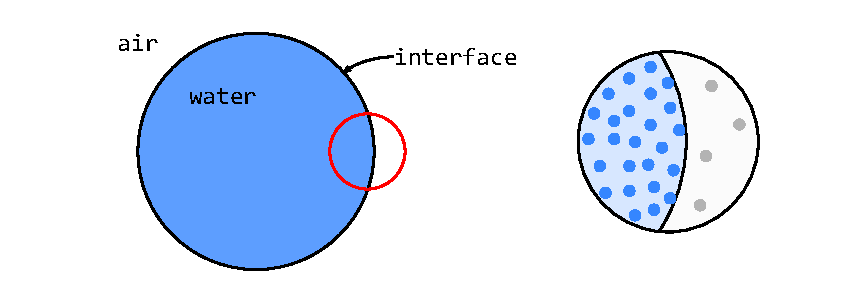
\includegraphics[width=.9\textwidth]{Pictures/moleculesAhesionCohesion_Wetting.pdf}
    \caption{Schematic of interacting molecules in a liquid droplet and its interaction with a vapor}
    \label{fig: WettingTheory_SurfaceTensionMolecules}
\end{figure}
To increase the surface area, molecules must be transported to the surface, and energy must be supplied to the system. Therefore, surface tension is also interpreted as the necessary energy required to carry a molecule to the surface.
\begin{equation}
    dE = \sigma \cdot dA
\end{equation}
with \(dE\) as the supplied energy and \(dA\) as the change in surface area.


\section{Wetting Phenomenon}
Despite the fact that the wetting of droplets is not considered in this work, it is appropriate to describe the fundamentals of wetting using this example. The concepts are the same, and many initial studies are based on this example.

In the case where the system is in equilibrium, Young \cite{youngIIIEssayCohesion1805} derived an equation relating surface tensions to the contact angle:
\begin{equation}
    \sigma_{\mathrm{LV}} \cdot \cos\theta_{\mathrm{e}} = \sigma_{\mathrm{SV}}-\sigma_{\mathrm{SL}}
    \label{eq: YoungsEQ}
\end{equation}
Where $\sigma_{\mathrm{LV}}$ is the surface tension between the liquid and the gas, $\sigma_{\mathrm{SV}}$ is from the solid to the gas, and $\sigma_{\mathrm{SL}}$ is between the solid and the liquid (see Figure \ref{fig: YoungsLaw_ThreePhaseContactLine}).
\begin{figure}[h]
    \centering
    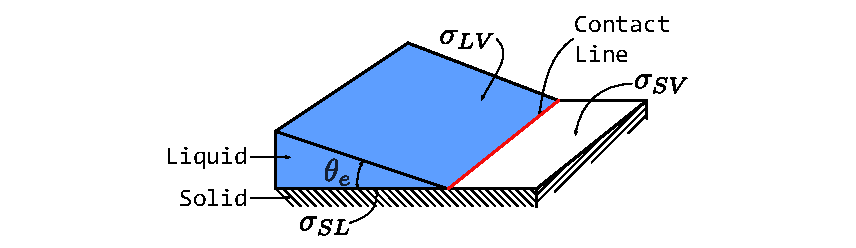
\includegraphics[width=.9\textwidth]{Pictures/YoungsLaw.pdf}
    \caption{Three Phase Contact Line}
    \label{fig: YoungsLaw_ThreePhaseContactLine}
\end{figure}
If $(\sigma_{\mathrm{SV}}>\sigma_{\mathrm{SL}})$ holds true, a contact angle less than $90^{\circ}$ follows; otherwise, $90^{\circ}\leq \theta_{\mathrm{e}}<180^{\circ}$. In the case where $\sigma_{\mathrm{SV}}=\sigma_{\mathrm{SL}}+\sigma_{\mathrm{LV}}$, complete wetting of the surface occurs \cite{buttPhysicsChemistryInterfaces}.

When a droplet impacts a solid surface, different states can arise depending on the fluid-solid combination. At the point where the interface of the two fluids (droplet and surrounding fluid) meets the solid surface, the contact line is formed (see \ref{fig: YoungsLaw_ThreePhaseContactLine}; red line). Depending on the fluid-fluid-solid combination, a contact angle $\theta_{\mathrm{e}}$ is established, where the suffix $e$ stands for equilibrium. In the case of complete wetting, the fluid spreads over the entire surface (see Figure \ref{fig: WettingTheory_WettingOfSurface} a)). This effect, however, is challenging to reproduce as it can be hindered by surface irregularities \cite{buttPhysicsChemistryInterfaces}. As seen in Figure \ref{fig: WettingTheory_WettingOfSurface}(b-d)), states where a droplet forms on the surface are further subdivided. For a contact angle $\theta_{\mathrm{e}}<90^{\circ}$, it is termed hydrophilic (see \ref{fig: WettingTheory_WettingOfSurface}b)), for $\theta_{\mathrm{e}}>90^{\circ}$ it's hydrophobic (see \ref{fig: WettingTheory_WettingOfSurface}c)), and for a contact angle $\theta_{\mathrm{e}}>120^{\circ}$, it's superhydrophobic surfaces (see \ref{fig: WettingTheory_WettingOfSurface}d)). Developing superhydrophobic surfaces is also challenging.
\begin{figure}[h]
    \centering
    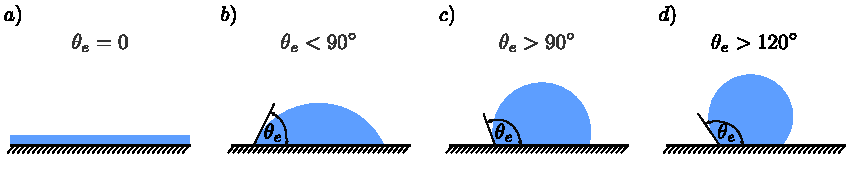
\includegraphics[width=.95\textwidth]{Pictures/DropletsAndWetting.pdf}
    \caption{Wetting of a surface}
    \label{fig: WettingTheory_WettingOfSurface}
\end{figure}
To curve the surface of the liquid, a pressure difference must exist. In the case of a sphere, Young and Laplace developed a relationship for the pressure difference in terms of the surface tension and radius as:
\begin{equation}
\label{eq: YoungLaplaceEQ}
    P_{\mathrm{i}} - P_{\mathrm{o}} = \Delta P =  \frac{2\sigma}{R}
\end{equation}
With $\Delta P$ being the pressure difference at the interface, $P_{\mathrm{i}}$ as the pressure inside the droplet, $P_{\mathrm{o}}$ the ambient pressure, and $R$ as the radius of the sphere. For a derivation, refer to \cite{buttPhysicsChemistryInterfaces}.


\subsection{Dynamic Weting}
So far, only states have been considered that observe systems in equilibrium. Typically, however, the contact line is in motion. When the contact line is moving, the contact angle (dynamic contact angle $\theta_{\mathrm{D}}$) differs from that in the equilibrium state \cite{blake2006PhysicsMovingWetting}. To describe the dynamics of the contact line, the dynamic contact angle, the relative speed of the contact line, and the equilibrium contact angle are required \cite{mohammadkarim2022ReviewPhysicsMoving, blake2006PhysicsMovingWetting, cox1986DynamicsSpreadingLiquids,huh1971HydrodynamicModelSteady,voinovHydrodynamicsWetting1977}. However, describing the contact line is challenging due to the fact that the microscopic level affects the macroscopic level.

In Figure \ref{fig: HDT_MKT_comp}, various views of the contact line are illustrated. The red circle in \textit{a)} points to the area considered in the picture next to it and can be understood as a magnifying glass. If we enlarge the area in \textit{a)}, we see the interpretation of the contact line from the perspective of the hydrodynamic theory, with a microscopic contact angle $\theta_{\mathrm{m}}$ and the dynamic contact angle $\theta_{\mathrm{D}}$ (Figure \ref{fig: HDT_MKT_comp} \textit{b)}). Focusing again on the contact line, we see the interpretation of the molecular kinetic theory (Figure \ref{fig: HDT_MKT_comp} \textit{c)}). The illustrated points are intended to represent molecules in a simplified form.




\begin{figure}[h]
    \centering
    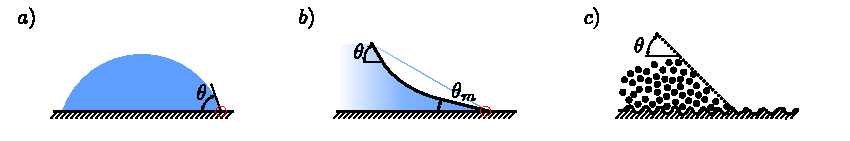
\includegraphics[width=.95\textwidth]{Pictures/ContactAngles_HDT_MKT.pdf}
    \caption{Hydrodynamic and Molecular Kinetic description of the Contact angle. Figure b) corresponds to the area circled in red in a), and c) to the area from image b).}
    \label{fig: HDT_MKT_comp}
\end{figure}

\paragraph{Hydrodynamic Theory}
\label{paragraph: hydrodynTheory}
The hydrodynamic approach solves the physics of the flow using the Navier-Stokes equations but encounters a singularity at the contact line when a sticking condition is applied \cite{huh1971HydrodynamicModelSteady}. To address this issue, either the sticking condition near the wall was relaxed or the solution was truncated at the molecular level \cite{blake2006PhysicsMovingWetting}. In both cases, a small capillary number is assumed, which means that far from the contact line, the interface assumes its equilibrium shape.

Voinov \cite{voinovHydrodynamicsWetting1977} derived a description of the contact line for a spreading droplet depending on the capillary number. A generalized version was developed by Cox \cite{cox1986DynamicsSpreadingLiquids} with some correction terms \cite{carlsonCapillarityDynamicWetting2012,blake2006PhysicsMovingWetting}. Thus, the dynamic contact angle for $\theta_{\mathrm{D}} \leq 3/4 \pi$ is given by
\begin{equation}
    \label{eq: Cox-Voinov}
    \theta_D^3-\theta_m^3= 9 Ca \ln\left(\frac{L}{L_m}\right) = 9 \frac{\mu u}{\sigma}\ln\left(\frac{L}{L_m}\right)
\end{equation}
With $L$ as the macroscopic path length and $L_{\mathrm{m}}$ as the microscopic path length. Assuming that the interface assumes its equilibrium shape far away, $\theta_{\mathrm{m}} = \theta_{\mathrm{e}}$. However, Voinov himself already pointed out that $\theta_{\mathrm{m}}$ could also depend on the speed \cite{voinovHydrodynamicsWetting1977,blake2006PhysicsMovingWetting,lacisNanoscaleShearedDroplet2022}.


\paragraph{Molecular Kinetic Theory}
The Molecular Kinetic Model describes the movement of the contact line with a statistical description of the molecular movement at the contact line \cite{blake1969KineticsDisplacement}. 
In contrast to the hydrodynamic model, the molecular processes at the contact line influence those of the larger scales. In this view, the molecules at the contact line jump back and forth to adsorption sites on the solid substrate. The speed of the contact line is determined by multiplying the difference between the forward and backward jumps by a jump distance $\lambda$. This results in the description
\begin{equation}
    u=2\lambda\kappa_{0}\sinh\left(\frac{\sigma\left(\cos\theta_{\mathrm{e}}-\cos\theta_{\mathrm{D}}\right)}{2nk_{\mathrm{B}}T}\right).
\end{equation}
Where $n$ is the number of adsorption sites per unit area, $k_0$ is a characteristic frequency, $k_{\mathrm{B}}$ is the Boltzmann constant, and $T$ is the temperature.
If the system is in equilibrium, the forward and backward jumping is balanced, and the contact line comes to a standstill \cite{carlson2011DissipationRapidDynamic,blake2006PhysicsMovingWetting}. However, a problem with this view is that this model is more qualitative and computationally intensive \cite{mohammadkarim2022ReviewPhysicsMoving}.








\subsection{Capillary Rise}
\label{sec: capillaryRise}
A capillary is a very thin tube in which, due to surface effects, a liquid rises or falls without external force. In \ref{fig: classicCapillary}, a capillary with an already risen liquid column is shown. The well-known surface tensions are also marked at their respective locations, as well as the essential geometric parameters, such as diameter ($2R$) or height of the resulting meniscus $z$. The resulting contact angle after reaching equilibrium, $\theta_{\mathrm{e}}$, is also shown. The system in this representation is also subject to gravitational forces.

\begin{figure}[h]
    \centering
    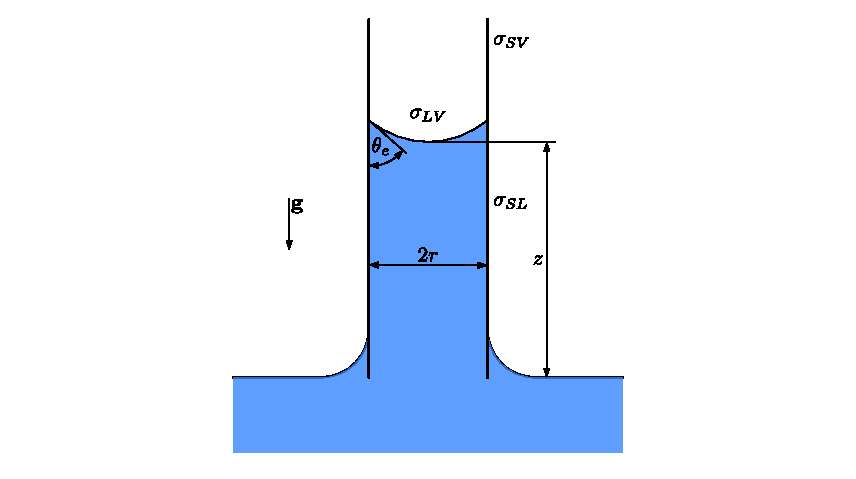
\includegraphics[width=.95\textwidth]{Pictures/classicCapillary.pdf}
    \caption{Schematic representation of a capillary in a liquid after it has penetrated the capillary.}
    \label{fig: classicCapillary}
\end{figure}

In this work, such a system is used. However, further conditions apply. It is assumed that the system is isobaric, isothermal, and the liquid is Newtonian. Furthermore, it is assumed that while the water column rises in the capillary, a Poiseuille flow is present and no phase change occurs. It is also assumed that the viscosity of the gas phase is negligible. With these assumptions and boundary conditions, the Newtonian dynamics in a capillary can be described as a balance between the inertial forces and the sum of the capillary forces, viscous forces, and hydrostatic forces \cite{fricke2023AnalyticalStudyCapillary}:

\begin{equation}
\label{eq: NewtonBalanceForcesOnly}
    \frac{d}{dt}M(z,\dot{z}) = F_{\mathrm{w}} - F_{\eta} - F_{\mathrm{g}}
\end{equation}

With $M(z,\dot{z}) = \pi r^2 \rho z \dot{z}$ as the moment, $F_{\mathrm{g}} = \pi r^2 \rho g z$ as the gravitational force, and $F_{\eta}$ as the viscous resistance, which results from the assumption of the average velocity and the existing Poiseuille flow to $F_{\eta}=8\pi\eta z \dot{z}$. With $\dot{z}$ as the average velocity. The capillary forces result from the previous description of the surface tension and the change in the surface of the meniscus with a change in the current height:

\begin{equation}
    F_{\mathrm{w}}=\sigma \frac{dA}{dz} = \sigma 2\pi r
\end{equation}

The surface tension $\sigma$ here is the increase in surface energy due to the wetting of the solid wall of the capillary. Thus, $\sigma = \sigma_{\mathrm{SV}}- \sigma_{\mathrm{SL}}$. This description is already known from the Young equation (\ref{eq: YoungsEQ}). Thus, after inserting for the capillary forces:

\begin{equation}
    F_W = \sigma_{\mathrm{LV}} \cdot \cos \theta_{\mathrm{e}} 2\pi r.
\end{equation}

Thus, for equation \ref{eq: NewtonBalanceForcesOnly} after insertion \cite{fricke2023AnalyticalStudyCapillary}:

\begin{equation}
\label{eq: NewtonDynCapillary}
    \pi r^2 \rho \frac{d}{dt} (z \dot{z}) = \sigma_{\mathrm{LV}} \cdot \cos \theta_{\mathrm{e}} 2\pi r-8\pi\eta z \dot{z}-\pi r^2 \rho g z.
\end{equation}

Early descriptions by Bell and Cameron \cite{bell1906FlowLiquidsCapillary} did not describe the rise dynamics based on equation \ref{eq: NewtonDynCapillary}. They developed the rise dynamics from experiments according to:

\begin{equation}
    z(t)^n = K\cdot t.
\end{equation}

Both $n$ and $K$ are temperature-dependent constants. In 1918, Lucas \cite{lucas1918UeberZeitgesetzKapillaren} and in 1921, Washburn \cite{washburn1921DynamicsCapillaryFlow} derived the Lucas Washburn equation by neglecting the inertial and gravitational terms:

\begin{equation}
\label{eq: LW-Eq}
    z(t) = \sqrt{\frac{r\sigma\cos\theta_{\mathrm{e}}}{2\eta}t}
\end{equation}

With this, they independently developed an equation with which the capillary rise can be described based on material values and measurements. Therefore, it gained popularity over the years. Due to the neglect of individual terms and simplifications in the system, however, this equation is not always precise for several reasons. Washburn himself pointed out that to meet the prediction of the equation, he had to set up the experiments in such a way that the capillary was prewetted. Therefore, adjustments to this equation were made for various problems \cite{dimitrov2007CapillaryRiseNanopores, heiranian2022ModifiedLucasWashburnTheory,cai2021LucasWashburnEquationBased,fries2008AnalyticSolutionCapillary,fricke2023AnalyticalStudyCapillary,delannoy2019DualRoleViscosity,martic2002MolecularDynamicsSimulation}. Wu et al. \cite{wu2017CapillaryRiseValidity} examined several models and compared them with experiments. In these, however, it is always assumed that the height of the meniscus increases according to $z(t)\sim \sqrt{t}$ as well.

Bosanquet \cite{bosanquet1923LVFlowLiquids} hinted in his 1923 paper that equation \ref{eq: LW-Eq} would lead to unphysical behavior for $t\xrightarrow{}0$ and also developed an equation that retained this problem but now also included inertia and can give a better prediction of the rise for early times of imbibition, but also fails for small capillary \cite{chen2023InvestigatingValidityBosanquet}. 

Siegel \cite{siegel1961TransientCapillaryRise} studied the rise behavior under microgravity and found a linear growth. However, he did not reach the Lucas-Washburn regime. Zhmud et al. \cite{zhmud2000DynamicsCapillaryRise} also pointed out the problems for times near $0$ from equation \ref{eq: LW-Eq} and described a quadratic relationship for the times when the fluid is drawn into the capillary, followed by the known Lucas-Washburn regime.

Dreyer et al. \cite{dreyer1994CapillaryRiseLiquid} studied parallel plates under microgravity and divided the rise of the meniscus into three regions. Starting with a quadratic growth, followed by a linear region, and finally the Lucas-Washburn growth. Quéré \cite{quere1997InertialCapillarity} showed a linear growth at the beginning by assuming that in this case only inertia plays a role. Stange \cite{stange2003CapillaryDrivenFlow} confirmed the three regions of Dreyer et al. \cite{dreyer1994CapillaryRiseLiquid} and derived dimensionless equations to develop transition times.

Fries et al. \cite{fries2008TransitionInertialViscous} divided the growth area into areas where different forces act. In the beginning, inertia dominates, followed by a transition area where the viscous forces take over until they finally dominate. They also developed dimensionless times at which the transition takes place.

At the point where the viscous friction and the effects of inertia or dynamic contact angle are equal, Quéré \cite{quere1997InertialCapillarity} and Fries et al. \cite{fries2008TransitionInertialViscous} defined the characteristic penetration length:
\begin{equation}
    \label{eq: charLength}
    l_{\mathrm{c}} \propto r \sqrt{\frac{r\rho \sigma}{\mu^2}}
\end{equation}
Dellanoy et al. \cite{delannoy2019DualRoleViscosity} focused on early times and studied viscous fluids, confirming the influence of pre-wetting the capillary, as already mentioned by Washburn \cite{washburn1921DynamicsCapillaryFlow}. They also showed a deviation from the Lucas-Washburn regime at early times. They attributed this deviation to local viscous dissipation in the wedge region, rather than a global dissipation as assumed by Lucas and Washburn. Regarding the dynamic contact angle, they showed that the characteristic penetration length (cf. Equation \ref{eq: charLength}) is calculated as:
\begin{equation}
    l_{\mathrm{c}} \propto r \ln\left(\frac{r}{l_{\mathrm{m}}}\right)
\end{equation}

With $l_m$ being the microscopic length that compensates for the singularity of the contact line \cite{cox1986DynamicsSpreadingLiquids}. They further assumed that once $l_c$ is reached, the transition to the Lucas-Washburn regime occurs.

Ruiz-Gutiérrez et al. \cite{ruiz-gutierrez2022LongCrossoverDynamics} contradicted this statement in their work, showing that this transition takes longer. They argue that the effects of inertia and dynamic contact angle do not decay exponentially. 

To account for this, they expanded Equation \ref{eq: NewtonDynCapillary} for problems with a moving interface by introducing:
\begin{equation}
    f(\dot{z}) \equiv \frac{\cos\theta_{\mathrm{m}}-\cos\theta_D(\dot{z})}{\cos\theta_{\mathrm{m}}} 
\end{equation}
With the assumption that for $u>0$ from Equation \ref{eq: Cox-Voinov}, $\theta_{\mathrm{D}} > \theta_{\mathrm{m}}$ holds true, this function disappears for $\theta_{\mathrm{D}} \rightarrow \theta_{\mathrm{m}}$. 

Now, considering the moving system, Equation \ref{eq: NewtonDynCapillary} for the case studied in this work becomes:
\begin{equation}
    \pi r^{2}\rho z \frac{du}{dt}= 2\pi r\sigma \cos\theta_{\mathrm{m}}+\pi r^{2}\rho gz-8\pi \sigma z \dot{z} -2\pi r \sigma \cos \theta_{\mathrm{m}}f
\end{equation}
With the first two terms as driving forces and the last two as resistance forces. The last term has been added and acts as a correction for the fact that the dynamic contact angle does not correspond to the macroscopic contact angle. \todo{is that so????}
For later usage the here proposed force, that is dissipated due to the formatation of the meniscus is given by:
\begin{equation}
    \label{eq: meniscusFormation}
    F_{\mathrm{m}} = 2\pi r \sigma (\cos \theta_{\mathrm{e}}-\cos \theta_{\mathrm{D}}(U))
\end{equation}

Subsequently, dimensionless quantities were introduced, and four cases were defined. Two each with a large and small Laplace number, or a large and small ratio of length scales. With the quantities used in this work, case three from Ruiz-Gutiérrez et al. \cite{ruiz-gutierrez2022LongCrossoverDynamics} should apply. They predict that the quadratic regime will not occur, and the rise will begin with a linear region, eventually transitioning to the Lucas-Washburn regime.


\todo[inline]{maybe use this eq instead of shorted one?}
\begin{equation}
    \pi r^2\rho l\frac{\mathrm{d}u}{\mathrm{d}t}=2\pi r\gamma\cos\theta_{\mathrm{a}}+\pi r^2\rho gh-8\pi\mu lu-\frac{3}{2}\pi r^2\rho u^2-2\pi r\gamma\cos\theta_{\mathrm{a}}f
\end{equation}


\section{Simulating the Wetting Processes}
Simulating a two-phase flow can be achieved through several methods. Common approaches include the \texttt{Volume-of-Fluid} and the \texttt{Level-Set} methods. Both methods use a sharp interface and are based on the Hydrodynamic Theory from Chapter \ref{paragraph: hydrodynTheory}. Moreover, they are \textit{interface capturing} methods, so they don't require recalculating the computational grid over the simulation period. Other methods that follow the interface (\textit{interface tracking}) are also possible. One of the major drawbacks of these methods is that the moving contact line, when using the adhesion condition, depends on models \cite{carlsonCapillarityDynamicWetting2012}. Additionally, calculating the surface tension can pose a challenge. This requires computing the curvature of the surface, which can lead to relatively high numerical errors \cite{jamshidi2019SuitabilityPhasefieldAlgebraic,hagg2019DirekteNumerischeSimulation}.

The Lattice-Boltzmann Method uses collision models to describe fluid behavior. Surface tensions can be considered through modifications. There are approaches that are promising and some are comparable to the phase-field method. However, one of the biggest challenges is the limitation of density or viscosity ratios. In this work, the fluids have significantly different densities with a ratio of $1000$. According to \cite{chenCriticalReviewPseudopotential2014}, the Lattice-Boltzmann Method is limited to ratios of $\mathcal{O}(10)$ and can lead to instabilities otherwise.

Another frequently used method is \texttt{Molecular Dynamic} simulations. Since individual molecules are simulated in this case, this method is only applicable to geometrically and temporally small problems without driving computational costs too high. Therefore, \texttt{Molecular Dynamic} simulations are often used for comparison or to study only small problems (\cite{datta2023EarlyStageLiquidInfiltration,lacisNanoscaleShearedDroplet2022,martic2002MolecularDynamicsSimulation,dimitrov2007CapillaryRiseNanopores}).

The method used in this work is the \texttt{phase-field} method. This method models two or even multi-phase flow through the system's free energy. A more detailed description of this method and the simulations already carried out is provided in Chapter \ref{chap: PhaseFieldMethod}. \todo[inline]{Elaborate or maybe move the entire section to phase field? Or perhaps case setup with a reasoning why phase field?}

